% Options for packages loaded elsewhere
\PassOptionsToPackage{unicode}{hyperref}
\PassOptionsToPackage{hyphens}{url}
%
\documentclass[
  man,floatsintext]{apa6}
\usepackage{amsmath,amssymb}
\usepackage{iftex}
\ifPDFTeX
  \usepackage[T1]{fontenc}
  \usepackage[utf8]{inputenc}
  \usepackage{textcomp} % provide euro and other symbols
\else % if luatex or xetex
  \usepackage{unicode-math} % this also loads fontspec
  \defaultfontfeatures{Scale=MatchLowercase}
  \defaultfontfeatures[\rmfamily]{Ligatures=TeX,Scale=1}
\fi
\usepackage{lmodern}
\ifPDFTeX\else
  % xetex/luatex font selection
\fi
% Use upquote if available, for straight quotes in verbatim environments
\IfFileExists{upquote.sty}{\usepackage{upquote}}{}
\IfFileExists{microtype.sty}{% use microtype if available
  \usepackage[]{microtype}
  \UseMicrotypeSet[protrusion]{basicmath} % disable protrusion for tt fonts
}{}
\makeatletter
\@ifundefined{KOMAClassName}{% if non-KOMA class
  \IfFileExists{parskip.sty}{%
    \usepackage{parskip}
  }{% else
    \setlength{\parindent}{0pt}
    \setlength{\parskip}{6pt plus 2pt minus 1pt}}
}{% if KOMA class
  \KOMAoptions{parskip=half}}
\makeatother
\usepackage{xcolor}
\usepackage{longtable,booktabs,array}
\usepackage{calc} % for calculating minipage widths
% Correct order of tables after \paragraph or \subparagraph
\usepackage{etoolbox}
\makeatletter
\patchcmd\longtable{\par}{\if@noskipsec\mbox{}\fi\par}{}{}
\makeatother
% Allow footnotes in longtable head/foot
\IfFileExists{footnotehyper.sty}{\usepackage{footnotehyper}}{\usepackage{footnote}}
\makesavenoteenv{longtable}
\usepackage{graphicx}
\makeatletter
\def\maxwidth{\ifdim\Gin@nat@width>\linewidth\linewidth\else\Gin@nat@width\fi}
\def\maxheight{\ifdim\Gin@nat@height>\textheight\textheight\else\Gin@nat@height\fi}
\makeatother
% Scale images if necessary, so that they will not overflow the page
% margins by default, and it is still possible to overwrite the defaults
% using explicit options in \includegraphics[width, height, ...]{}
\setkeys{Gin}{width=\maxwidth,height=\maxheight,keepaspectratio}
% Set default figure placement to htbp
\makeatletter
\def\fps@figure{htbp}
\makeatother
\setlength{\emergencystretch}{3em} % prevent overfull lines
\providecommand{\tightlist}{%
  \setlength{\itemsep}{0pt}\setlength{\parskip}{0pt}}
\setcounter{secnumdepth}{-\maxdimen} % remove section numbering
% Make \paragraph and \subparagraph free-standing
\ifx\paragraph\undefined\else
  \let\oldparagraph\paragraph
  \renewcommand{\paragraph}[1]{\oldparagraph{#1}\mbox{}}
\fi
\ifx\subparagraph\undefined\else
  \let\oldsubparagraph\subparagraph
  \renewcommand{\subparagraph}[1]{\oldsubparagraph{#1}\mbox{}}
\fi
\newlength{\cslhangindent}
\setlength{\cslhangindent}{1.5em}
\newlength{\csllabelwidth}
\setlength{\csllabelwidth}{3em}
\newlength{\cslentryspacingunit} % times entry-spacing
\setlength{\cslentryspacingunit}{\parskip}
\newenvironment{CSLReferences}[2] % #1 hanging-ident, #2 entry spacing
 {% don't indent paragraphs
  \setlength{\parindent}{0pt}
  % turn on hanging indent if param 1 is 1
  \ifodd #1
  \let\oldpar\par
  \def\par{\hangindent=\cslhangindent\oldpar}
  \fi
  % set entry spacing
  \setlength{\parskip}{#2\cslentryspacingunit}
 }%
 {}
\usepackage{calc}
\newcommand{\CSLBlock}[1]{#1\hfill\break}
\newcommand{\CSLLeftMargin}[1]{\parbox[t]{\csllabelwidth}{#1}}
\newcommand{\CSLRightInline}[1]{\parbox[t]{\linewidth - \csllabelwidth}{#1}\break}
\newcommand{\CSLIndent}[1]{\hspace{\cslhangindent}#1}
\ifLuaTeX
\usepackage[bidi=basic]{babel}
\else
\usepackage[bidi=default]{babel}
\fi
\babelprovide[main,import]{english}
% get rid of language-specific shorthands (see #6817):
\let\LanguageShortHands\languageshorthands
\def\languageshorthands#1{}
% Manuscript styling
\usepackage{upgreek}
\captionsetup{font=singlespacing,justification=justified}

% Table formatting
\usepackage{longtable}
\usepackage{lscape}
% \usepackage[counterclockwise]{rotating}   % Landscape page setup for large tables
\usepackage{multirow}		% Table styling
\usepackage{tabularx}		% Control Column width
\usepackage[flushleft]{threeparttable}	% Allows for three part tables with a specified notes section
\usepackage{threeparttablex}            % Lets threeparttable work with longtable

% Create new environments so endfloat can handle them
% \newenvironment{ltable}
%   {\begin{landscape}\centering\begin{threeparttable}}
%   {\end{threeparttable}\end{landscape}}
\newenvironment{lltable}{\begin{landscape}\centering\begin{ThreePartTable}}{\end{ThreePartTable}\end{landscape}}

% Enables adjusting longtable caption width to table width
% Solution found at http://golatex.de/longtable-mit-caption-so-breit-wie-die-tabelle-t15767.html
\makeatletter
\newcommand\LastLTentrywidth{1em}
\newlength\longtablewidth
\setlength{\longtablewidth}{1in}
\newcommand{\getlongtablewidth}{\begingroup \ifcsname LT@\roman{LT@tables}\endcsname \global\longtablewidth=0pt \renewcommand{\LT@entry}[2]{\global\advance\longtablewidth by ##2\relax\gdef\LastLTentrywidth{##2}}\@nameuse{LT@\roman{LT@tables}} \fi \endgroup}

% \setlength{\parindent}{0.5in}
% \setlength{\parskip}{0pt plus 0pt minus 0pt}

% Overwrite redefinition of paragraph and subparagraph by the default LaTeX template
% See https://github.com/crsh/papaja/issues/292
\makeatletter
\renewcommand{\paragraph}{\@startsection{paragraph}{4}{\parindent}%
  {0\baselineskip \@plus 0.2ex \@minus 0.2ex}%
  {-1em}%
  {\normalfont\normalsize\bfseries\itshape\typesectitle}}

\renewcommand{\subparagraph}[1]{\@startsection{subparagraph}{5}{1em}%
  {0\baselineskip \@plus 0.2ex \@minus 0.2ex}%
  {-\z@\relax}%
  {\normalfont\normalsize\itshape\hspace{\parindent}{#1}\textit{\addperi}}{\relax}}
\makeatother

% \usepackage{etoolbox}
\makeatletter
\patchcmd{\HyOrg@maketitle}
  {\section{\normalfont\normalsize\abstractname}}
  {\section*{\normalfont\normalsize\abstractname}}
  {}{\typeout{Failed to patch abstract.}}
\patchcmd{\HyOrg@maketitle}
  {\section{\protect\normalfont{\@title}}}
  {\section*{\protect\normalfont{\@title}}}
  {}{\typeout{Failed to patch title.}}
\makeatother

\usepackage{xpatch}
\makeatletter
\xapptocmd\appendix
  {\xapptocmd\section
    {\addcontentsline{toc}{section}{\appendixname\ifoneappendix\else~\theappendix\fi\\: #1}}
    {}{\InnerPatchFailed}%
  }
{}{\PatchFailed}
\keywords{Methodology, Meta-analysis, Development, Online studies\newline\indent Word count: X}
\usepackage{lineno}

\linenumbers
\usepackage{csquotes}
\ifLuaTeX
  \usepackage{selnolig}  % disable illegal ligatures
\fi
\IfFileExists{bookmark.sty}{\usepackage{bookmark}}{\usepackage{hyperref}}
\IfFileExists{xurl.sty}{\usepackage{xurl}}{} % add URL line breaks if available
\urlstyle{same}
\hypersetup{
  pdftitle={Conducting developmental research online vs.~in-person: A meta-analysis},
  pdfauthor={Aaron Chuey1, Veronica Boyce1, Anjie Cao1, \& Michael C. Frank1},
  pdflang={en-EN},
  pdfkeywords={Methodology, Meta-analysis, Development, Online studies},
  hidelinks,
  pdfcreator={LaTeX via pandoc}}

\title{Conducting developmental research online vs.~in-person: A meta-analysis}
\author{Aaron Chuey\textsuperscript{1}, Veronica Boyce\textsuperscript{1}, Anjie Cao\textsuperscript{1}, \& Michael C. Frank\textsuperscript{1}}
\date{}


\shorttitle{Conducting developmental research online}

\authornote{

The authors made the following contributions. Aaron Chuey: Conceptualization, Methodology, Formal analysis, Data Curation, Visualization, Writing - Original Draft; Veronica Boyce: Conceptualization, Methodology, Formal analysis, Data Curation, Visualization, Writing - Review \& Editing; Anjie Cao: Conceptualization, Methodology, Formal analysis, Data Curation, Visualization, Writing - Review \& Editing; Michael C. Frank: Conceptualization, Methodology, Formal analysis, Data Curation, Visualization, Writing - Review \& Editing, Supervision.

Correspondence concerning this article should be addressed to Aaron Chuey. E-mail: \href{mailto:chuey@stanford.edu}{\nolinkurl{chuey@stanford.edu}}

}

\affiliation{\vspace{0.5cm}\textsuperscript{1} Stanford University, Department of Psychology}

\abstract{%
An increasing number of psychological experiments with children are being conducted using online platforms, in part due to the COVID-19 pandemic. Individual replications have compared the findings of particular experiments online and in-person, but the general effect of data collection method on data collected from children is still unknown. Therefore, the goal of the current meta-analysis is to estimate the average difference in effect size for developmental studies conducted online compared to the same studies conducted in-person. Our pre-registered analysis includes 211 effect sizes calculated from 30 papers with 3282 children, ranging in age from four months to six years. The mean effect size of studies conducted online were slightly larger than the mean effect size of their counterparts conducted in-person, a mean difference of d=-.12, but this difference was not significant, 95\% CI={[}-.34, .09{]}. We examined several potential moderators of the effect of online testing, including the role of dependent measure (looking vs verbal), online study method (moderated vs unmoderated), and age, but none of these were significant. The literature to date thus suggests -- on average -- small differences in results between in-person and online experimentation for young children.
}



\begin{document}
\maketitle

\hypertarget{introduction}{%
\section{Introduction}\label{introduction}}

Developmental researchers are interested in studying children's behavior, primarily by measuring their behavioral responses to experimental stimuli. Study sessions typically involve visits with local families in a laboratory setting or partnering with remote sites such as schools and museums. Although these interactions are a routine part of developmental research, they are time-consuming for both researchers and participants. Typical studies with dozens of infants or young children can require weeks or months of scheduling visits to a lab or many visits to testing sites. In-person testing also limits the participant pool to children living relatively close to the research site. Additionally, developmental research has been plagued by small, non-diverse samples even more so than research with adults due to limitations imposed by the demographics of the local population as well as the high costs of collecting data from children (Kidd \& Garcia, 2022; Nielsen et al., 2017).

Prior to the rise of video chat software, there were only limited alternatives to in-person interaction for collecting experimental behavioral data from children. However, with the development of inexpensive and reliable video conferencing technology in the 2010s, new frontiers began to emerge for developmental testing.\footnote{Observational and survey research has long been conducted through the phone or by mail (e.g., Fenson et al., 1994); here we focus primarily on behavioral observation and experimental methods.} Indeed, even infants appear to follow others' gaze (Capparini et al., 2023) and establish joint attention over video chat (McClure et al., 2018). Researchers soon experimented with conducting developmental studies through video-chat platforms, which in theory broaden the pool of participants to anyone at nearly any time and location so long as they have access to internet and an internet enabled device. What began as a few research teams experimenting with online studies (e.g., Lookit: Scott \& Schulz, 2017; The Child Lab: Sheskin \& Keil, 2018; Pandas: Rhodes et al., 2020) quickly expanded to much of the field as researchers scrambled to conduct safe research during the Covid-19 pandemic. This shift in research practices has yielded many empirical publications where some or all of the data were collected online. In addition, there is a growing literature on online methodology and best practices for designing such studies (we will not review this guidance here, but see e.g., Chuey, Asaba, et al., 2021; Kominsky, Begus, et al., 2021).

Some researchers may be eager to return to in-person testing, but online research is likely here to stay and may increase in frequency as communications technologies improve and become more accessible. Online testing has immense potential to change developmental science (Sheskin et al., 2020), much as crowdsourced testing of adults has changed adult behavioral science (Buhrmester et al., 2016). This potential has yet to be fully realized, however, as researchers have yet to fully understand the strengths and weaknesses of this method, as well as how to recruit diverse populations for online studies. Despite undersampling certain populations (Lourenco \& Tasimi, 2020), online studies nonetheless allow researchers to sample from a larger, broader pool of participants than ever before as access to the internet continues to increase worldwide. Large, low cost samples and remote cross-cultural research may even become a reality for developmental researchers in the coming years.

How different are the results of developmental studies conducted online to those conducted in person? Direct comparison of effects measured in both modalities is critical to answering this question. Researchers have implemented a number of paradigms online and replicated their in-person findings, but it is still largely unknown how the quality of data yielded from online developmental studies more broadly compares to those conducted in-person. Therefore, the current meta-analysis seeks to estimate effect sizes for phenomena measured with children online and for the same phenomena measured in closely-matched in-person studies. These study pairs in turn allow estimation of the average magnitude of the difference between in-person and online studies.

On the one hand, there is good reason to suspect that modality has little influence over the strength of a study's effect. Fundamentally, studies conducted online and in-person utilize similar measures (e.g., looking time, verbal report) and use similar kinds of stimuli (e.g., moving objects, narrated vignettes). Additionally, experimenters still need to contend with extraneous factors like inattention, environmental distractions, and participants' mood. On the other hand, meaningful differences in online and in-person interactions could affect the outcomes of online and in-person studies, in either direction.

In principle, researchers have more control over a child's environment in-person, and in-person studies are usually less susceptible to technical problems such as lag or auditory or visual fidelity issues. Conversely, participants typically complete online studies in a more comfortable, familiar environment -- their own home. Any of these factors could tip the scales, yielding larger effects in-person or online; as a result, we do not make any predictions regarding the presence or direction of an effect of study modality. Further, there are many ways in which online studies vary including whether a live experimenter is present, what the dependent measure is (e.g., preferential looking vs.~reaching), and the age of the sample being tested. Such factors could also influence the outcomes of online and in-person studies.

Online studies are generally conducted in one of two formats: moderated or unmoderated. In moderated studies, a live experimenter guides participants through a study much like they would in-person, except online, typically via video-chat. Moderated studies are often operationalized as slides or videos shared with participants while the participants' verbal responses or gaze is recorded. In contrast, with unmoderated studies participants complete a study without the guidance of a live experimenter. Instead, researchers create a preprogrammed module that participants or their caregivers initiate and complete according to instructions. Since no experimenter needs to be present and participants can participate at any time they choose, unmoderated studies offer the potential for fast, inexpensive data collection. However, since they lack an experimenter, participants' experiences also deviate more from in-person studies compared to moderated studies that retain the same core social interaction between experimenter and participant. Therefore, it is possible that data collected via unmoderated sessions is comparatively noisier since an experimenter is unable to focus children's attention or course correct like they can during a live interaction. We consider this possibility in the current meta-analysis.

Like developmental studies more broadly, online studies have also employed a number of dependent measures, including verbal and looking measures. Verbal measures are typically straightforward to record, while recording looking measures is more complex. Accurate looking measures require precise camera positioning and coding schemes, and are thus more likely to deviate from their in-person counterparts compared to studies that measure children's verbal responses. To that end, automated gaze annotation is currently being developed and represents an exciting future direction in online methodology (Chouinard et al., 2019; see Erel et al., 2022; Steffan et al., 2024). We examine how the kind of dependent measure employed (looking vs.~verbal) might moderate the difference between online and in-person results.

The final moderator we consider is participants' age. Online developmental studies have sampled from a wide age range, including infants (e.g., Dillon et al., 2020), toddlers (e.g., Lo et al., 2021), preschoolers (e.g., Schidelko et al., 2021), and elementary schoolers (e.g., Chuey et al., 2020; Chuey, McCarthy, et al., 2021). Because online studies are often conducted in the comfort of their own homes, it is possible that children of all ages might benefit from this aspect of online studies. Conversely, because a child's environment is more difficult to moderate online, infant studies, which often rely on precise environmental setups, may suffer more when conducted online. In addition, as children get older they may gain more experience with on-screen displays, which can contribute to their performance in online studies. We test these competing age moderation hypotheses.

In sum, to estimate the average effect size associated with online study administration for young children, we conducted a meta-analysis of matched studies conducted online and in-person; this includes online studies that replicated an older study conducted in-person as well as pairs of online and in-person studies conducted in parallel. In addition, we asked whether these differences are moderated by study format, dependent variable, or participant age.

We stress that our goal here is not to provide a conclusive, binary answer to the question of whether online and in-person studies are the same or different. Likely with enough studies to analyze, we would find that there are many cases when they are similar and some where they are different. Instead, our goal is to provide a best guess as to, on average, how different an effect would be if it was measured online vs.~in-person. Even if there is some uncertainty in this estimate due to heterogeneity and the limited number of available comparative studies, we believe it is an important piece of information for developmental researchers as they plan the modality of their next study.

\hypertarget{methods}{%
\section{Methods}\label{methods}}

\begin{figure}
\centering
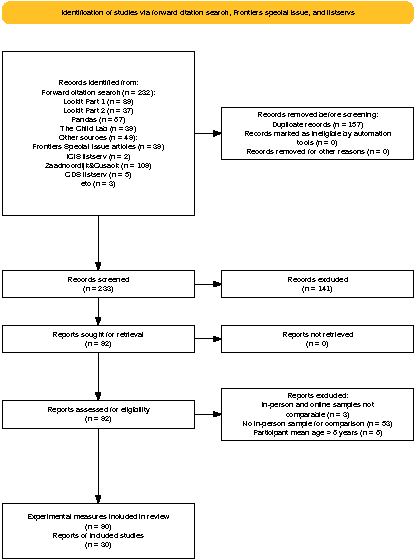
\includegraphics{OnlineMA_main_files/figure-latex/prisma-1.pdf}
\caption{\label{fig:prisma}PRISMA plot detailing our study screening process; numerical values represent the number of papers at each stage of the systematic search.}
\end{figure}

We conducted a literature search following the Preferred Reporting Items for Systematic Reviews and Meta-Analyses (PRISMA) procedure (Page et al., 2021); see Figure \ref{fig:prisma}. For each set of studies determined to be an online replication, we calculated the effect size(s) and associated variance for the main effect of interest. We then conducted a series of random-effects multilevel meta-regressions to estimate the effect of online data collection, as well as three possible moderators (online study method, type of dependent measure, and participant age). Our preregistered data selection, coding, and analysis plan can be found at \href{}{https://osf.io/hjbxf}. The list of papers included in this meta-analysis is shown in Table \ref{tab:list}.

\hypertarget{literature-search}{%
\subsection{Literature Search}\label{literature-search}}

Our goal was to find as many published and unpublished online replications of developmental studies as possible. However, because there is no common nomenclature for online replications and the studies themselves cover a wide range of research questions and methodologies, searching via specific terms or keywords was difficult and produced many irrelevant papers; as a result, we could not conduct a completely systematic review. Instead, we preregistered a forward citation search strategy based on key papers on online developmental research. We used the papers that conducted initial validation of popular online testing platforms as our seeds, including Lookit (Scott et al., 2017; Scott \& Schulz, 2017), The Child Lab (Sheskin \& Keil, 2018), and Pandas (Rhodes et al., 2020). Any paper that cited at least one of these papers was considered for inclusion in our meta-analysis. We also considered all papers published in the Frontiers in Psychology Special Issue: Empirical Research at a Distance: New Methods for Developmental Science, which largely focused on online developmental studies and replications. Additionally, we were were pointed to (Zaadnoordijk \& Cusack, 2022) which contained a list of online replication papers, although this yielded few additional replications. Finally, we posted a call for contributions to the Cognitive Development Society (CDS) and International Congress of Infant Studies (ICIS) listservs, two popular emailing lists frequented by developmental researchers. This call yielded several publications our initial search strategy missed, as well as six unpublished but complete online replications.

We preregistered several eligibility criteria to filter articles from our search:

\begin{enumerate}
\def\labelenumi{\arabic{enumi}.}
\item
  The study must be experimental, where participants complete a task with a stimulus. This criterion precludes surveys or purely observational measures.
\item
  The studies must report two groups of children, one tested online and another tested in-person. Although the online sample must be collected by the researchers reporting the results, the in-person sample could either be collected at the same time or referenced from an existing publication.
\item
  The mean age of the sample should be under six years. This criterion limits the studies to those conducted on relatively younger children for whom online data collection methods have not been traditionally employed.
\item
  All data reported or referred to must contain codable effect sizes. Verbal comparison alone between an online or in-person study or a qualitative description of results is not enough to determine the precise effect size of interest.
\item
  Data collection for both the in-person and online sample must be complete; any incomplete or partial samples were not considered.
\item
  The online and in-person methods must be directly comparable. Some alteration to the study methods is expected when adapting an in-person study to be run online (e.g., having children refer to objects by color instead of pointing). However, we excluded any studies whose methodologies altered the nature of the task or the conclusions that could be drawn from them (e.g., changing the identity of a hidden object instead of its location in a false belief task).
\end{enumerate}

\begin{longtable}[]{@{}
  >{\raggedright\arraybackslash}p{(\columnwidth - 8\tabcolsep) * \real{0.7961}}
  >{\raggedleft\arraybackslash}p{(\columnwidth - 8\tabcolsep) * \real{0.0583}}
  >{\raggedright\arraybackslash}p{(\columnwidth - 8\tabcolsep) * \real{0.0485}}
  >{\raggedright\arraybackslash}p{(\columnwidth - 8\tabcolsep) * \real{0.0583}}
  >{\raggedleft\arraybackslash}p{(\columnwidth - 8\tabcolsep) * \real{0.0388}}@{}}
\caption{\label{tab:list}Papers used in this meta-analysis, ordered by average participant age (in months). Some papers contained both online and in-person results, others contained online replications compared to previous in-person papers. Pairs refers to the number of paired online and in-person effect sizes contributed by each paper (set). Look is whether the studies use looking, verbal, or both types of dependent measures. Mod is whether the online studies were moderated, unmoderated, or both.}\tabularnewline
\toprule\noalign{}
\begin{minipage}[b]{\linewidth}\raggedright
Paper
\end{minipage} & \begin{minipage}[b]{\linewidth}\raggedleft
Pairs
\end{minipage} & \begin{minipage}[b]{\linewidth}\raggedright
Look
\end{minipage} & \begin{minipage}[b]{\linewidth}\raggedright
Mod
\end{minipage} & \begin{minipage}[b]{\linewidth}\raggedleft
Age
\end{minipage} \\
\midrule\noalign{}
\endfirsthead
\toprule\noalign{}
\begin{minipage}[b]{\linewidth}\raggedright
Paper
\end{minipage} & \begin{minipage}[b]{\linewidth}\raggedleft
Pairs
\end{minipage} & \begin{minipage}[b]{\linewidth}\raggedright
Look
\end{minipage} & \begin{minipage}[b]{\linewidth}\raggedright
Mod
\end{minipage} & \begin{minipage}[b]{\linewidth}\raggedleft
Age
\end{minipage} \\
\midrule\noalign{}
\endhead
\bottomrule\noalign{}
\endlastfoot
Gasparini et al. (2022) & 5 & Verb & Mod & 4 \\
Bánki et al. (2022) & 4 & Look & Unmod & 5 \\
DeJesus et al. (2021) & 3 & Verb & Mod & 5 \\
McElwain et al. (2022) & 27 & Both & Mod & 6 \\
Bochynska and Dillon (2021) compared to Dillon et al. (2020) & 2 & Look & Unmod & 7 \\
Bulgarelli and Bergelson (2022) & 3 & Look & Mod & 8 \\
Yuen and Hamlin (2022) compared to Hamlin (2015) & 2 & Both & Mod & 9 \\
Beckner et al. (2023) & 1 & Look & Unmod & 9 \\
Smith-Flores et al. (2022) compared to Stahl and Feigenson (2015) & 3 & Look & Mod & 13 \\
Smith-Flores (2022) compared to Skerry and Spelke (2014) & 2 & Look & Mod & 13 \\
Lo et al. (2021) & 1 & Verb & Unmod & 19 \\
Margoni et al. (2018) & 2 & Look & Mod & 21 \\
Steffan et al. (2023) & 1 & Look & Mod & 22 \\
Nguyen et al. (2022) & 2 & Verb & Mod & 22 \\
Chuey, Asaba, et al. (2021) & 3 & Both & Mod & 24 \\
Mani (2022) & 1 & Look & Mod & 24 \\
Morini and Blair (2021) & 1 & Verb & Mod & 30 \\
Silver et al. (2021) & 1 & Verb & Mod & 33 \\
Schidelko et al. (2021) & 4 & Verb & Mod & 44 \\
Lapidow et al. (2021) & 4 & Verb & Both & 44 \\
Scott et al. (2017) compared to Téglás et al. (2007) and Pasquini et al. (2007) & 17 & Both & Unmod & 45 \\
Yoon and Frank (2019) & 2 & Verb & Unmod & 48 \\
Kominsky, Shafto, et al. (2021) & 1 & Verb & Mod & 55 \\
Escudero et al. (2021) & 2 & Verb & Mod & 57 \\
Vales et al. (2021) & 3 & Verb & Mod & 58 \\
Nelson et al. (2021) & 8 & Verb & Mod & 59 \\
Gerard (2022) & 1 & Verb & Unmod & 60 \\
Wang and Roberts (2023) & 1 & Verb & Mod & 60 \\
Aboody, Huey, et al. (2022) & 1 & Verb & Mod & 60 \\
Aboody, Yousif, et al. (2022) & 1 & Verb & Mod & 72 \\
\end{longtable}

\hypertarget{data-entry}{%
\subsection{Data Entry}\label{data-entry}}

All papers (233) yielded by our search procedure went through three rounds of evaluation to determine if they met our inclusion criteria. First, we screened the titles of the papers to determine whether they might include an online experiment. Those that clearly did not meet one or more of our inclusion criteria were excluded from further evaluation. Next, we performed a similar evaluation based on the papers' abstracts, before a final round based on the article as a whole. All remaining papers were entered into a spreadsheet that coded the necessary information for calculating the size of the main effect(s) of interest and their associated variance (sample size, group means and standard deviation, and t and F statistics when applicable), as well as our preregistered moderators (study modality, data collection method, dependent measure, and participant age).

If a paper reported an effect size as Cohen's d (referred to below as standardized mean difference, SMD), we coded it directly. Otherwise, we calculated the individual effect sizes for each main effect and each study (online and in-person) via reported means and standard deviations, t-statistic, or directly from the data if it was available using analysis scripts adapted from Metalab (e.g., Bergmann et al., 2018), a repository of meta-analyses in early language and cognitive development. If the main comparison was to chance performance, we first calculated log odds and then converted the effect size to cohen's d via the compute.es package in R (Del Re \& Del Re, 2012). If a given study had multiple dependent measures or central hypotheses, we calculated an effect size and associated variance for each.

\hypertarget{analytic-approach}{%
\subsection{Analytic Approach}\label{analytic-approach}}

To determine whether study modality (online or in-person) moderated the size of the main effect of interest for each set of studies, we performed a preregistered random-effects multilevel meta-regression using the metafor package in R (Viechtbauer, 2010). The regression predicted individual study effect size (SMD) with study modality as a fixed effect, modeling individual experimental effect sizes with the coefficient of interest being the study modality predictor (online vs.~in-person). As discussed above, we did not predict a direction of effect for the study modality predictor.

Our approach focused on the study modality moderator, rather than computing an online-offline difference score for each study and estimating the size of that difference directly. Although at a first glance this approach may seem simpler, many papers are heterogeneous and contain multiple online studies for a single given offline study, or multiple measures within the same study. In these cases, the appropriate difference was not always clear. For this reason, we chose to enter all study effects into the meta-regression and use the study modality moderator to estimate systematic modality effects.

To ensure that differences in the total number of effect sizes across studies did not bias our analysis by overweighting studies with more measurements, we included two random intercepts in our models. The first random intercept captured variation between particular experiments (e.g., modeling the dependency between multiple measurements reported from a single experiment). The second captured variation between groups of participants (e.g., modeling the dependency between effect sizes from participants who completed a battery of tasks with multiple effects of interest).

To determine the effect of additional moderators -- online study method (moderated vs unmoderated), dependent measure (looking vs verbal), and participant age - we conducted three additional multilevel meta-regressions each with an additional fixed effect plus the corresponding interaction with study modality. All analysis scripts were preregistered, and the code is available at \href{}{https://osf.io/up6qn}.

\hypertarget{results}{%
\section{Results}\label{results}}

\begin{table}[!h]

\caption{\label{tab:coeffs}Table of coefficients for the pre-registered models. The overall model is shown first, followed by the three models with moderators.}
\centering
\begin{tabular}[t]{lrlr}
\toprule
Coefficient & Estimate & 95\% CI & P-value\\
\midrule
\addlinespace[0.3em]
\multicolumn{4}{l}{\textbf{Overall}}\\
\hspace{1em}Intercept & 0.75 & {}[0.4, 1.09] & 0.000\\
\hspace{1em}Online & -0.12 & {}[-0.34, 0.09] & 0.254\\
\addlinespace[0.3em]
\multicolumn{4}{l}{\textbf{Looking v Verbal}}\\
\hspace{1em}Intercept & 0.65 & {}[0.49, 0.82] & 0.000\\
\hspace{1em}Online & -0.15 & {}[-0.39, 0.09] & 0.227\\
\hspace{1em}Verbal & -0.05 & {}[-0.13, 0.04] & 0.292\\
\hspace{1em}Online:Verbal & 0.04 & {}[-0.14, 0.21] & 0.693\\
\addlinespace[0.3em]
\multicolumn{4}{l}{\textbf{Age}}\\
\hspace{1em}Intercept & 0.62 & {}[0.46, 0.78] & 0.000\\
\hspace{1em}Online & -0.14 & {}[-0.37, 0.08] & 0.207\\
\hspace{1em}Age & 0.00 & {}[-0.01, 0.01] & 0.843\\
\hspace{1em}Online:Age & 0.00 & {}[-0.01, 0.01] & 0.526\\
\addlinespace[0.3em]
\multicolumn{4}{l}{\textbf{Moderated v Un-moderated}}\\
\hspace{1em}Intercept & 0.62 & {}[0.47, 0.78] & 0.000\\
\hspace{1em}Online & -0.16 & {}[-0.4, 0.08] & 0.193\\
Unmoderated & 0.11 & {}[-0.22, 0.43] & 0.515\\
\bottomrule
\end{tabular}
\end{table}

\begin{figure}[h]

{\centering 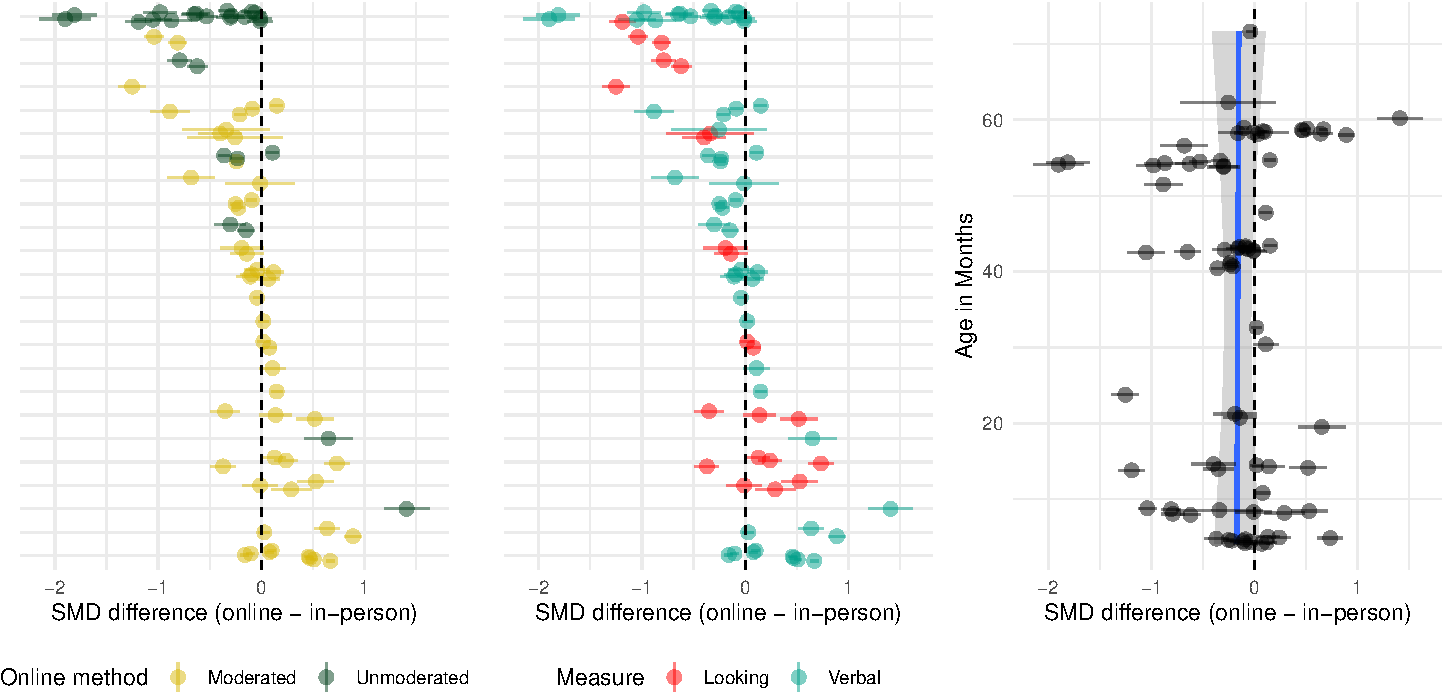
\includegraphics[width=1\linewidth]{OnlineMA_main_files/figure-latex/forest-1} 

}

\caption{Forest plots of studies, sorted by difference in SMD. Each row is one study (paper or pair of papers) and contains every effect size pair contributed by that study. Each dot represents the difference between a single in-person measure and a corresponding online measure. A: Difference in SMD by study and online method (moderated vs unmoderated). B: Difference in SMD by study and measurement type (looking vs verbal). C: Difference in SMD by study and mean participant age (months).}\label{fig:forest}
\end{figure}

\hypertarget{planned-analysis}{%
\subsection{Planned Analysis}\label{planned-analysis}}

Overall, the meta-analysis revealed a small negative, non-significant effect of online study modality, Est=-0.12, 95\% CI={[}-0.34, 0.09{]}, p=0.254. Additionally, we did not find any significant effect of our preregistered moderators or any significant interactions between the moderators and study modality. See Table \ref{tab:coeffs} for coefficient values. Figure \ref{fig:forest} shows the effect size differences of experiments by moderators.

Because our meta-analysis averaged across effects from very different paradigms (which could yield different effect sizes independent of the effect of testing modality), we expected substantial heterogeneity. Consistent with that expectation, all tests for residual heterogeneity were highly significant (all \(p\)s \(< .0001\)). Values of \(\tau^2\) (the between-study variance in our meta-analysis) for all models were 0.23 (primary model), 0.23 (moderated vs.~unmoderated model), 0.23 (looking-time model), and 0.23 (age model), respectively, confirming the impression that these moderators did not reduce heterogeneity.

\hypertarget{exploratory-analysis}{%
\subsection{Exploratory Analysis}\label{exploratory-analysis}}

\begin{longtable}[]{@{}
  >{\raggedright\arraybackslash}p{(\columnwidth - 10\tabcolsep) * \real{0.1370}}
  >{\raggedright\arraybackslash}p{(\columnwidth - 10\tabcolsep) * \real{0.1644}}
  >{\raggedright\arraybackslash}p{(\columnwidth - 10\tabcolsep) * \real{0.1096}}
  >{\raggedleft\arraybackslash}p{(\columnwidth - 10\tabcolsep) * \real{0.3014}}
  >{\raggedleft\arraybackslash}p{(\columnwidth - 10\tabcolsep) * \real{0.0822}}
  >{\raggedright\arraybackslash}p{(\columnwidth - 10\tabcolsep) * \real{0.2055}}@{}}
\caption{\label{tab:modmeans}Mean SMD across studies by study modality, data-collection method, and type of dependent measure}\tabularnewline
\toprule\noalign{}
\begin{minipage}[b]{\linewidth}\raggedright
Modality
\end{minipage} & \begin{minipage}[b]{\linewidth}\raggedright
Method
\end{minipage} & \begin{minipage}[b]{\linewidth}\raggedright
Measure
\end{minipage} & \begin{minipage}[b]{\linewidth}\raggedleft
N (Effect-size Pairs)
\end{minipage} & \begin{minipage}[b]{\linewidth}\raggedleft
SMD
\end{minipage} & \begin{minipage}[b]{\linewidth}\raggedright
95\% CI
\end{minipage} \\
\midrule\noalign{}
\endfirsthead
\toprule\noalign{}
\begin{minipage}[b]{\linewidth}\raggedright
Modality
\end{minipage} & \begin{minipage}[b]{\linewidth}\raggedright
Method
\end{minipage} & \begin{minipage}[b]{\linewidth}\raggedright
Measure
\end{minipage} & \begin{minipage}[b]{\linewidth}\raggedleft
N (Effect-size Pairs)
\end{minipage} & \begin{minipage}[b]{\linewidth}\raggedleft
SMD
\end{minipage} & \begin{minipage}[b]{\linewidth}\raggedright
95\% CI
\end{minipage} \\
\midrule\noalign{}
\endhead
\bottomrule\noalign{}
\endlastfoot
In-person & Moderated & Looking & 15 & 0.752 & {[}0.439, 1.065{]} \\
In-person & Moderated & Verbal & 34 & 0.492 & {[}0.286, 0.698{]} \\
Online & Moderated & Looking & 12 & 0.573 & {[}0.264, 0.882{]} \\
Online & Moderated & Verbal & 27 & 0.372 & {[}0.218, 0.525{]} \\
Online & Unmoderated & Looking & 5 & 0.214 & {[}0.062, 0.367{]} \\
Online & Unmoderated & Verbal & 6 & 1.227 & {[}0.285, 2.169{]} \\
\end{longtable}

In addition to our multi-level meta-analysis, we examined which combinations of methods and measures tended to yield the strongest and weakest effect sizes relative to their in-person counterparts. We fit a meta-analytic model containing method, response mode, and modality as well as their two- and three-way interactions, with the same random effects structure as our previous model. We cannot draw any strong conclusions about these noisy estimates due to our relatively small sample size. That said, descriptively, unmoderated online studies with looking measures were estimated to have noticeably smaller effect sizes compared to both their moderated online and in-person counterparts (See Table \ref{tab:modmeans}). In contrast, as estimated by this model, moderated online studies with looking and verbal measures as well as unmoderated online studies with verbal measures did not show such large differences from their in-person counterparts.

\begin{figure}[h]

{\centering 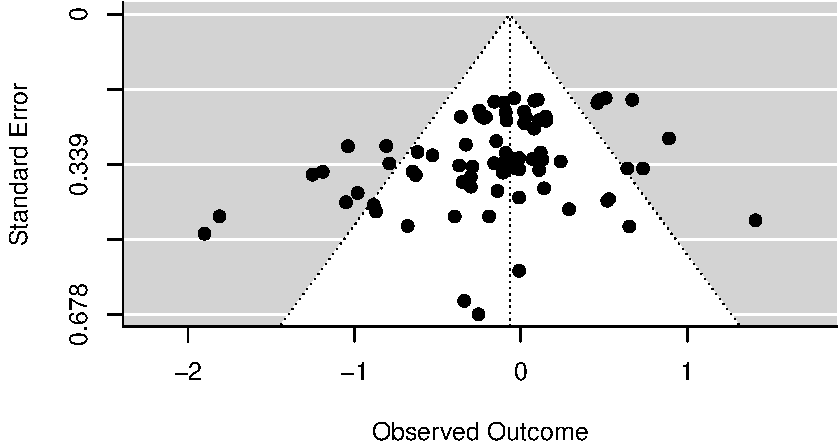
\includegraphics[width=0.8\linewidth]{OnlineMA_main_files/figure-latex/funnel-1} 

}

\caption{Funnel plot of the differences in effect size between pairs of in-person and online studies. A positive observed outcome means the online study had a larger effect size. \label{funnel}}\label{fig:funnel}
\end{figure}

We also conducted an exploratory analysis of potential publication bias. It was unclear \emph{a priori} how we might expect publication biases to manifest themselves, given that there is some possibility of notoriety for either showing \emph{or} failing to show differences between online and in-person testing. In either case our hypothesized selection process operated on the \emph{differences} in effect sizes between each online and in-lab pair of samples.

For each online and in-person pair on the same study, we calculated a standard mean difference in effect size between the two studies as well as the variance of this difference. The resulting funnel plot is shown in Figure \ref{fig:funnel}. As the difference in effect size increases, the variance should also increase; however, if asymmetries are observed in this relationship (e.g., a greater number of negative outcome values with low variance), effect sizes may not have been uniformly reported. According to Egger's regression test for funnel plot asymmetry, a common method for assessing publication bias in meta-analyses, this plot is asymmetric (p=.005) and the estimated effect assuming no variance is 0.26 {[}-0.03, 0.55{]}. This analysis suggests the possibility of publication bias favoring studies that have smaller effect sizes online compared to in-person, signaling that perhaps online studies may have relatively larger effect sizes on average compared to what has been reported. We interpret this conclusion with caution, however, noting the large width of the estimated CI and the relatively low power of Egger's test (Sterne et al., 2000).

\hypertarget{discussion}{%
\section{Discussion}\label{discussion}}

The current meta-analysis provides a birds-eye view of how developmental studies conducted online compare with closely matched counterparts conducted in-person. Our results suggest that overall, comparable studies yield relatively similar effect sizes. Even the upper end of the confidence interval for the online-offline difference estimate is still relatively small. This finding should be heartening for developmentalists interested in using online data collection.

We also examined whether modality effects emerged more substantially in particular settings, but did not find evidence for other moderators. The method of online data collection, type of dependent measure, and participant age did not have a significant impact on the effect of modality. Nonetheless, the lack of statistical precision, indicated by relatively wide confidence intervals, limits our ability to draw strong conclusions about the effect of any of our moderators. Future analysis is needed to determine the moderating effect, if any, that these factors exercise on the outcome of developmental studies conducted online.

The current analysis is coarse-grained, considering only one particular dichotomy within study modality: in-person vs online. Yet, there are many ways that developmental studies can be further subdivided. For example, studies are conducted both in quiet spaces (e.g., in lab, at home) and loud spaces (e.g., parks, museums), although the lack of granularity with respect to how these factors are reported in the literature renders us unable to examine them in the current meta-analysis. Therefore, online studies might over- or under-perform relative to studies conducted in particular in-person locations. Our moderators are also correspondingly course-grained, particularly dependent measure (looking vs verbal). Because our small sample size renders our analysis underpowered to detect weaker effects of moderators, the current results and their interpretation are subject to change as online methods improve and comparisons to in-person studies are better understood.

Unmoderated studies with looking measures had the noticeably smallest effect sizes relative to their in-person counterparts. This could reflect the difficulty of both collecting and coding looking data online using participants' own webcams without significant real-time instruction. Indeed, it is possible that effect sizes suffer without a live experimenter eliciting and sustaining infants' attention or guiding parents as they position and orient their infant. However, smaller effect sizes online could instead reflect genuinely smaller effect sizes of the underlying effect rather than a lack of online studies' sensitivity. Developmental research has suffered from many failures to replicate in the past, especially studies with infants (e.g., Davis-Kean \& Ellis, 2019), and many of the online studies in our sample were conducted after their in-person counterparts, sometimes years later. Therefore, it is possible that smaller online effect sizes simply represent a more accurate estimation of the true (smaller) effect rather than an effect of study modaility per se.

Unfortunately, the studies in our sample did not consistently report demographic information at the level of detail necessary for investigating how participants' home environment, socioeconomic status, or identity moderated the effect of study modality. Although children's demographic characteristics influence their study performance no matter the modality, these factors arguably stand to exert a greater influence over the outcome of online studies because in-person studies standardize the study environment across participants while online studies do not. Thus, the effect sizes of studies conducted online are additionally at the mercy of participants' home environment, and by extension the demographic factors that shape its features.

The composition of our sample might also bias our results. To match online and in-person methods as closely as possible, we only considered direct online replications for the current meta-analysis. While this approach ensures that data were collected online and in-person using similar methods and procedures, it limits our sample size and may bias our sample. For example, perhaps researchers disproportionately choose to conduct online replications of strong or well-established effects rather than replicate more subtle, weaker effects. Nonetheless, our analysis found that if publication bias exists, it likely favors stronger in-person effect sizes or non-replications among the studies we sampled. We also included an open call for unpublished data in an attempt to limit the file drawer problem (see Rosenthal, 1979).

Although developmental researchers have had decades of experience designing and running experiments in-person, most have only had a few years or less of experience developing online studies. Thus, our meta-analysis might also underestimate the potential of online research due to researcher and experimenter inexperience. Over the next several years, as developmental researchers develop expertise and experience with conducting research online, online studies might become more accurate at capturing cognitive constructs for any number of reasons, including better experimenter-participant interactions, better stimulus design (see Chuey, Asaba, et al., 2021), and more accurate methods of measurement (i.e., automatic looking time measures, see Erel et al., 2022). Relatedly, as new methods are developed and adapted for online experiments, researchers should not take the current findings as a blanket declaration that all online studies produce comparable results to their in-person counterparts; some might underperform, while others might outperform. Nonetheless, the current results suggest that across currently employed developmental methodologies, the effect sizes of studies conducted with children online are generally comparable to those conducted in-person, especially for studies utilizing verbal measures.

\hypertarget{conclusion}{%
\section{Conclusion}\label{conclusion}}

Our meta-analysis found that, across closely matched developmental studies conducted in-person and online, the size of the main effect of interest for in-person studies was similar to the effect for online studies, yielding only a small average difference between them. While our sample of studies limits the precision of our estimates, nevertheless the general similarity in outcomes for in-person and online studies with children paint an optimistic picture for online developmental research more broadly going forward.

\newpage

\hypertarget{references}{%
\section{References}\label{references}}

\hypertarget{refs}{}
\begin{CSLReferences}{1}{0}
\leavevmode\vadjust pre{\hypertarget{ref-aboody2022preschoolers}{}}%
Aboody, R., Huey, H., \& Jara-Ettinger, J. (2022). Preschoolers decide who is knowledgeable, who to inform, and who to trust via a causal understanding of how knowledge relates to action. \emph{Cognition}, \emph{228}, 105212.

\leavevmode\vadjust pre{\hypertarget{ref-aboody2022says}{}}%
Aboody, R., Yousif, S. R., Sheskin, M., \& Keil, F. C. (2022). Says who? Children consider informants' sources when deciding whom to believe. \emph{Journal of Experimental Psychology: General}.

\leavevmode\vadjust pre{\hypertarget{ref-banki2022comparing}{}}%
Bánki, A., Eccher, M. de, Falschlehner, L., Hoehl, S., \& Markova, G. (2022). Comparing online webcam-and laboratory-based eye-tracking for the assessment of infants' audio-visual synchrony perception. \emph{Frontiers in Psychology}, 6162.

\leavevmode\vadjust pre{\hypertarget{ref-beckner2023investigation}{}}%
Beckner, A. G., Voss, A. T., Phillips, L., King, K., Casasola, M., \& Oakes, L. M. (2023). An investigation of mental rotation in infancy using change detection. \emph{Infant Behavior and Development}, \emph{71}, 101834.

\leavevmode\vadjust pre{\hypertarget{ref-bergmann2018}{}}%
Bergmann, C., Tsuji, S., Piccinini, P. E., Lewis, M. L., Braginsky, M., Frank, M. C., \& Cristia, A. (2018). Promoting replicability in developmental research through meta-analyses: Insights from language acquisition research. \emph{Child Development}, \emph{89}(6), 1996--2009.

\leavevmode\vadjust pre{\hypertarget{ref-bochynska2021bringing}{}}%
Bochynska, A., \& Dillon, M. R. (2021). Bringing home baby euclid: Testing infants' basic shape discrimination online. \emph{Frontiers in Psychology}, 6002.

\leavevmode\vadjust pre{\hypertarget{ref-buhrmester2016amazon}{}}%
Buhrmester, M., Kwang, T., \& Gosling, S. D. (2016). \emph{Amazon's mechanical turk: A new source of inexpensive, yet high-quality data?}

\leavevmode\vadjust pre{\hypertarget{ref-bulgarelli2022talker}{}}%
Bulgarelli, F., \& Bergelson, E. (2022). Talker variability shapes early word representations in english-learning 8-month-olds. \emph{Infancy}, \emph{27}(2), 341--368.

\leavevmode\vadjust pre{\hypertarget{ref-capparini2023should}{}}%
Capparini, C., To, M. P., \& Reid, V. M. (2023). Should i follow your virtual gaze? Infants' gaze following over video call. \emph{Journal of Experimental Child Psychology}, \emph{226}, 105554.

\leavevmode\vadjust pre{\hypertarget{ref-chouinard2019using}{}}%
Chouinard, B., Scott, K., \& Cusack, R. (2019). Using automatic face analysis to score infant behaviour from video collected online. \emph{Infant Behavior and Development}, \emph{54}, 1--12.

\leavevmode\vadjust pre{\hypertarget{ref-chuey2021moderated}{}}%
Chuey, A., Asaba, M., Bridgers, S., Carrillo, B., Dietz, G., Garcia, T., Leonard, J. A., Liu, S., Merrick, M., Radwan, S., et al. (2021). Moderated online data-collection for developmental research: Methods and replications. \emph{Frontiers in Psychology}, 4968.

\leavevmode\vadjust pre{\hypertarget{ref-chuey2020children}{}}%
Chuey, A., Lockhart, K., Sheskin, M., \& Keil, F. (2020). Children and adults selectively generalize mechanistic knowledge. \emph{Cognition}, \emph{199}, 104231.

\leavevmode\vadjust pre{\hypertarget{ref-chuey2021no}{}}%
Chuey, A., McCarthy, A., Lockhart, K., Trouche, E., Sheskin, M., \& Keil, F. (2021). No guts, no glory: Underestimating the benefits of providing children with mechanistic details. \emph{Npj Science of Learning}, \emph{6}(1), 1--7.

\leavevmode\vadjust pre{\hypertarget{ref-davis2019overview}{}}%
Davis-Kean, P. E., \& Ellis, A. (2019). An overview of issues in infant and developmental research for the creation of robust and replicable science. \emph{Infant Behavior and Development}, \emph{57}, 101339.

\leavevmode\vadjust pre{\hypertarget{ref-dejesus2021young}{}}%
DeJesus, J. M., Venkatesh, S., \& Kinzler, K. D. (2021). Young children's ability to make predictions about novel illnesses. \emph{Child Development}, \emph{92}(5), e817--e831.

\leavevmode\vadjust pre{\hypertarget{ref-dillon2020infants}{}}%
Dillon, M. R., Izard, V., \& Spelke, E. S. (2020). Infants' sensitivity to shape changes in 2D visual forms. \emph{Infancy}, \emph{25}(5), 618--639.

\leavevmode\vadjust pre{\hypertarget{ref-erel2022icatcher}{}}%
Erel, Y., Potter, C. E., Jaffe-Dax, S., Lew-Williams, C., \& Bermano, A. H. (2022). iCatcher: A neural network approach for automated coding of young children's eye movements. \emph{Infancy}, \emph{27}(4), 765--779.

\leavevmode\vadjust pre{\hypertarget{ref-escudero2021four}{}}%
Escudero, P., Pino Escobar, G., Casey, C. G., \& Sommer, K. (2021). Four-year-old's online versus face-to-face word learning via eBooks. \emph{Frontiers in Psychology}, 450.

\leavevmode\vadjust pre{\hypertarget{ref-fenson1994variability}{}}%
Fenson, L., Dale, P. S., Reznick, J. S., Bates, E., Thal, D. J., Pethick, S. J., Tomasello, M., Mervis, C. B., \& Stiles, J. (1994). Variability in early communicative development. \emph{Monographs of the Society for Research in Child Development}, i--185.

\leavevmode\vadjust pre{\hypertarget{ref-gasparini2022online}{}}%
Gasparini, C., Caravale, B., Focaroli, V., Paoletti, M., Pecora, G., Bellagamba, F., Chiarotti, F., Gastaldi, S., \& Addessi, E. (2022). Online assessment of motor, cognitive, and communicative achievements in 4-month-old infants. \emph{Children}, \emph{9}(3), 424.

\leavevmode\vadjust pre{\hypertarget{ref-gerard2022extragrammaticality}{}}%
Gerard, J. (2022). The extragrammaticality of the acquisition of adjunct control. \emph{Language Acquisition}, \emph{29}(2), 107--134.

\leavevmode\vadjust pre{\hypertarget{ref-hamlin2015case}{}}%
Hamlin, J. (2015). The case for social evaluation in preverbal infants: Gazing toward one's goal drives infants' preferences for helpers over hinderers in the hill paradigm. \emph{Frontiers in Psychology}, \emph{5}, 1563.

\leavevmode\vadjust pre{\hypertarget{ref-kidd2022diverse}{}}%
Kidd, E., \& Garcia, R. (2022). How diverse is child language acquisition research? \emph{First Language}, 01427237211066405.

\leavevmode\vadjust pre{\hypertarget{ref-kominsky2021organizing}{}}%
Kominsky, J. F., Begus, K., Bass, I., Colantonio, J., Leonard, J. A., Mackey, A. P., \& Bonawitz, E. (2021). Organizing the methodological toolbox: Lessons learned from implementing developmental methods online. \emph{Frontiers in Psychology}, \emph{12}, 702710.

\leavevmode\vadjust pre{\hypertarget{ref-kominsky2021there}{}}%
Kominsky, J. F., Shafto, P., \& Bonawitz, E. (2021). {``There's something inside''}: Children's intuitions about animate agents. \emph{PloS One}, \emph{16}(5), e0251081.

\leavevmode\vadjust pre{\hypertarget{ref-lapidow2021tale}{}}%
Lapidow, E., Tandon, T., Goddu, M., \& Walker, C. M. (2021). A tale of three platforms: Investigating preschoolers' second-order inferences using in-person, zoom, and lookit methodologies. \emph{Frontiers in Psychology}, \emph{12}, 731404.

\leavevmode\vadjust pre{\hypertarget{ref-lo2021tablet}{}}%
Lo, C. H., Rosslund, A., Chai, J. H., Mayor, J., \& Kartushina, N. (2021). Tablet assessment of word comprehension reveals coarse word representations in 18--20-month-old toddlers. \emph{Infancy}, \emph{26}(4), 596--616.

\leavevmode\vadjust pre{\hypertarget{ref-lourenco2020no}{}}%
Lourenco, S. F., \& Tasimi, A. (2020). No participant left behind: Conducting science during COVID-19. \emph{Trends in Cognitive Sciences}, \emph{24}(8), 583--584.

\leavevmode\vadjust pre{\hypertarget{ref-mani2022}{}}%
Mani, N. (2022). \emph{Thematic priming}.

\leavevmode\vadjust pre{\hypertarget{ref-margoni2018infants}{}}%
Margoni, F., Baillargeon, R., \& Surian, L. (2018). Infants distinguish between leaders and bullies. \emph{Proceedings of the National Academy of Sciences}, \emph{115}(38), E8835--E8843.

\leavevmode\vadjust pre{\hypertarget{ref-mcclure2018look}{}}%
McClure, E. R., Chentsova-Dutton, Y. E., Holochwost, S. J., Parrott, W., \& Barr, R. (2018). Look at that! Video chat and joint visual attention development among babies and toddlers. \emph{Child Development}, \emph{89}(1), 27--36.

\leavevmode\vadjust pre{\hypertarget{ref-mcelwain2022zoom}{}}%
McElwain, N. L., Hu, Y., Li, X., Fisher, M. C., Baldwin, J. C., \& Bodway, J. M. (2022). Zoom, zoom, baby! Assessing mother-infant interaction during the still face paradigm and infant language development via a virtual visit procedure. \emph{Frontiers in Psychology}, \emph{12}, 734492.

\leavevmode\vadjust pre{\hypertarget{ref-morini2021webcams}{}}%
Morini, G., \& Blair, M. (2021). Webcams, songs, and vocabulary learning: A comparison of in-person and remote data collection as a way of moving forward with child-language research. \emph{Frontiers in Psychology}, 3347.

\leavevmode\vadjust pre{\hypertarget{ref-nelson2021comparing}{}}%
Nelson, P. M., Scheiber, F., Laughlin, H. M., \& Demir-Lira, Ö. (2021). Comparing face-to-face and online data collection methods in preterm and full-term children: An exploratory study. \emph{Frontiers in Psychology}, 5025.

\leavevmode\vadjust pre{\hypertarget{ref-nguyenadapting}{}}%
Nguyen, D., Fitzpatrick, N., \& Floccia, C. (2022). \emph{Adapting language development paradigms to online testing}.

\leavevmode\vadjust pre{\hypertarget{ref-nielsen2017persistent}{}}%
Nielsen, M., Haun, D., Kärtner, J., \& Legare, C. H. (2017). The persistent sampling bias in developmental psychology: A call to action. \emph{Journal of Experimental Child Psychology}, \emph{162}, 31--38.

\leavevmode\vadjust pre{\hypertarget{ref-page2021prisma}{}}%
Page, M. J., McKenzie, J. E., Bossuyt, P. M., Boutron, I., Hoffmann, T. C., Mulrow, C. D., Shamseer, L., Tetzlaff, J. M., Akl, E. A., Brennan, S. E., et al. (2021). The PRISMA 2020 statement: An updated guideline for reporting systematic reviews. \emph{International Journal of Surgery}, \emph{88}, 105906.

\leavevmode\vadjust pre{\hypertarget{ref-pasquini2007preschoolers}{}}%
Pasquini, E. S., Corriveau, K. H., Koenig, M., \& Harris, P. L. (2007). Preschoolers monitor the relative accuracy of informants. \emph{Developmental Psychology}, \emph{43}(5), 1216.

\leavevmode\vadjust pre{\hypertarget{ref-rhodes2020advancing}{}}%
Rhodes, M., Rizzo, M. T., Foster-Hanson, E., Moty, K., Leshin, R. A., Wang, M., Benitez, J., \& Ocampo, J. D. (2020). Advancing developmental science via unmoderated remote research with children. \emph{Journal of Cognition and Development}, \emph{21}(4), 477--493.

\leavevmode\vadjust pre{\hypertarget{ref-rosenthal1979file}{}}%
Rosenthal, R. (1979). The file drawer problem and tolerance for null results. \emph{Psychological Bulletin}, \emph{86}(3), 638.

\leavevmode\vadjust pre{\hypertarget{ref-schidelko2021online}{}}%
Schidelko, L. P., Schünemann, B., Rakoczy, H., \& Proft, M. (2021). Online testing yields the same results as lab testing: A validation study with the false belief task. \emph{Frontiers in Psychology}, 4573.

\leavevmode\vadjust pre{\hypertarget{ref-scott2017lookitB}{}}%
Scott, K., Chu, J., \& Schulz, L. (2017). Lookit (part 2): Assessing the viability of online developmental research, results from three case studies. \emph{Open Mind}, \emph{1}(1), 15--29.

\leavevmode\vadjust pre{\hypertarget{ref-scott2017lookit}{}}%
Scott, K., \& Schulz, L. (2017). Lookit (part 1): A new online platform for developmental research. \emph{Open Mind}, \emph{1}(1), 4--14.

\leavevmode\vadjust pre{\hypertarget{ref-sheskin2018thechildlab}{}}%
Sheskin, M., \& Keil, F. (2018). \emph{TheChildLab. Com a video chat platform for developmental research}.

\leavevmode\vadjust pre{\hypertarget{ref-sheskin2020online}{}}%
Sheskin, M., Scott, K., Mills, C. M., Bergelson, E., Bonawitz, E., Spelke, E. S., Fei-Fei, L., Keil, F. C., Gweon, H., Tenenbaum, J. B., et al. (2020). Online developmental science to foster innovation, access, and impact. \emph{Trends in Cognitive Sciences}, \emph{24}(9), 675--678.

\leavevmode\vadjust pre{\hypertarget{ref-silver2021measuring}{}}%
Silver, A. M., Elliott, L., Braham, E. J., Bachman, H. J., Votruba-Drzal, E., Tamis-LeMonda, C. S., Cabrera, N., \& Libertus, M. E. (2021). Measuring emerging number knowledge in toddlers. \emph{Frontiers in Psychology}, 3057.

\leavevmode\vadjust pre{\hypertarget{ref-skerry2014preverbal}{}}%
Skerry, A. E., \& Spelke, E. S. (2014). Preverbal infants identify emotional reactions that are incongruent with goal outcomes. \emph{Cognition}, \emph{130}(2), 204--216.

\leavevmode\vadjust pre{\hypertarget{ref-smith2022b}{}}%
Smith-Flores, A. S. (2022). \emph{Replication of skerry \& spelke (2014)}.

\leavevmode\vadjust pre{\hypertarget{ref-smith2022online}{}}%
Smith-Flores, A. S., Perez, J., Zhang, M. H., \& Feigenson, L. (2022). Online measures of looking and learning in infancy. \emph{Infancy}, \emph{27}(1), 4--24.

\leavevmode\vadjust pre{\hypertarget{ref-stahl2015observing}{}}%
Stahl, A. E., \& Feigenson, L. (2015). Observing the unexpected enhances infants' learning and exploration. \emph{Science}, \emph{348}(6230), 91--94.

\leavevmode\vadjust pre{\hypertarget{ref-steffan2023validation}{}}%
Steffan, A., Zimmer, L., Arias-Trejo, N., Bohn, M., Ben, R. D., Flores-Coronado, M. A., Franchin, L., Garbisch, I., Grosse Wiesmann, C., Hamlin, J. K., et al. (2023). \emph{Validation of an open source, remote web-based eye-tracking method (WebGazer) for research in early childhood}.

\leavevmode\vadjust pre{\hypertarget{ref-steffan2024validation}{}}%
Steffan, A., Zimmer, L., Arias-Trejo, N., Bohn, M., Dal Ben, R., Flores-Coronado, M. A., Franchin, L., Garbisch, I., Grosse Wiesmann, C., Hamlin, J. K., et al. (2024). Validation of an open source, remote web-based eye-tracking method (WebGazer) for research in early childhood. \emph{Infancy}, \emph{29}(1), 31--55.

\leavevmode\vadjust pre{\hypertarget{ref-sterne2000}{}}%
Sterne, J. A., Gavaghan, D., \& Egger, M. (2000). Publication and related bias in meta-analysis: Power of statistical tests and prevalence in the literature. \emph{Journal of Clinical Epidemiology}, \emph{53}(11), 1119--1129.

\leavevmode\vadjust pre{\hypertarget{ref-teglas2007intuitions}{}}%
Téglás, E., Girotto, V., Gonzalez, M., \& Bonatti, L. L. (2007). Intuitions of probabilities shape expectations about the future at 12 months and beyond. \emph{Proceedings of the National Academy of Sciences}, \emph{104}(48), 19156--19159.

\leavevmode\vadjust pre{\hypertarget{ref-vales2021research}{}}%
Vales, C., Wu, C., Torrance, J., Shannon, H., States, S. L., \& Fisher, A. V. (2021). Research at a distance: Replicating semantic differentiation effects using remote data collection with children participants. \emph{Frontiers in Psychology}, \emph{12}, 697550.

\leavevmode\vadjust pre{\hypertarget{ref-viechtbauer2010conducting}{}}%
Viechtbauer, W. (2010). Conducting meta-analyses in r with the metafor package. \emph{Journal of Statistical Software}, \emph{36}(3), 1--48.

\leavevmode\vadjust pre{\hypertarget{ref-wang2023being}{}}%
Wang, M. M., \& Roberts, S. O. (2023). Being from a highly resourced context predicts believing that others are highly resourced: An early developing worldview that stymies resource sharing. \emph{Journal of Experimental Child Psychology}, \emph{230}, 105624.

\leavevmode\vadjust pre{\hypertarget{ref-yoon2019preschool}{}}%
Yoon, E. J., \& Frank, M. C. (2019). Preschool children's understanding of polite requests. \emph{CogSci}, 3179--3185.

\leavevmode\vadjust pre{\hypertarget{ref-yuen2022}{}}%
Yuen, F., \& Hamlin, K. (2022). \emph{Replication of hamlin (2015)}.

\leavevmode\vadjust pre{\hypertarget{ref-zaadnoordijk2022online}{}}%
Zaadnoordijk, L., \& Cusack, R. (2022). Online testing in developmental science: A guide to design and implementation. In \emph{Advances in child development and behavior} (Vol. 62, pp. 93--125). Elsevier.

\end{CSLReferences}


\end{document}
